\chapter{Particle Simulator}
\label{chap:particle-simulator}

The aforementioned many-body systems generally exert very complex behaviour when viewed as a whole.
This behaviour can be captured in mathematical terms but also from a simulation perspective.
Particle simulations have been a subject of much attention in physics and scientific computing more generally.
This class of simulations, in the context of intermolecular interactions, is often referred to as molecular dynamics.

\begin{figure}[H]
  \centering
  \label{fig:simulation-quiver}
  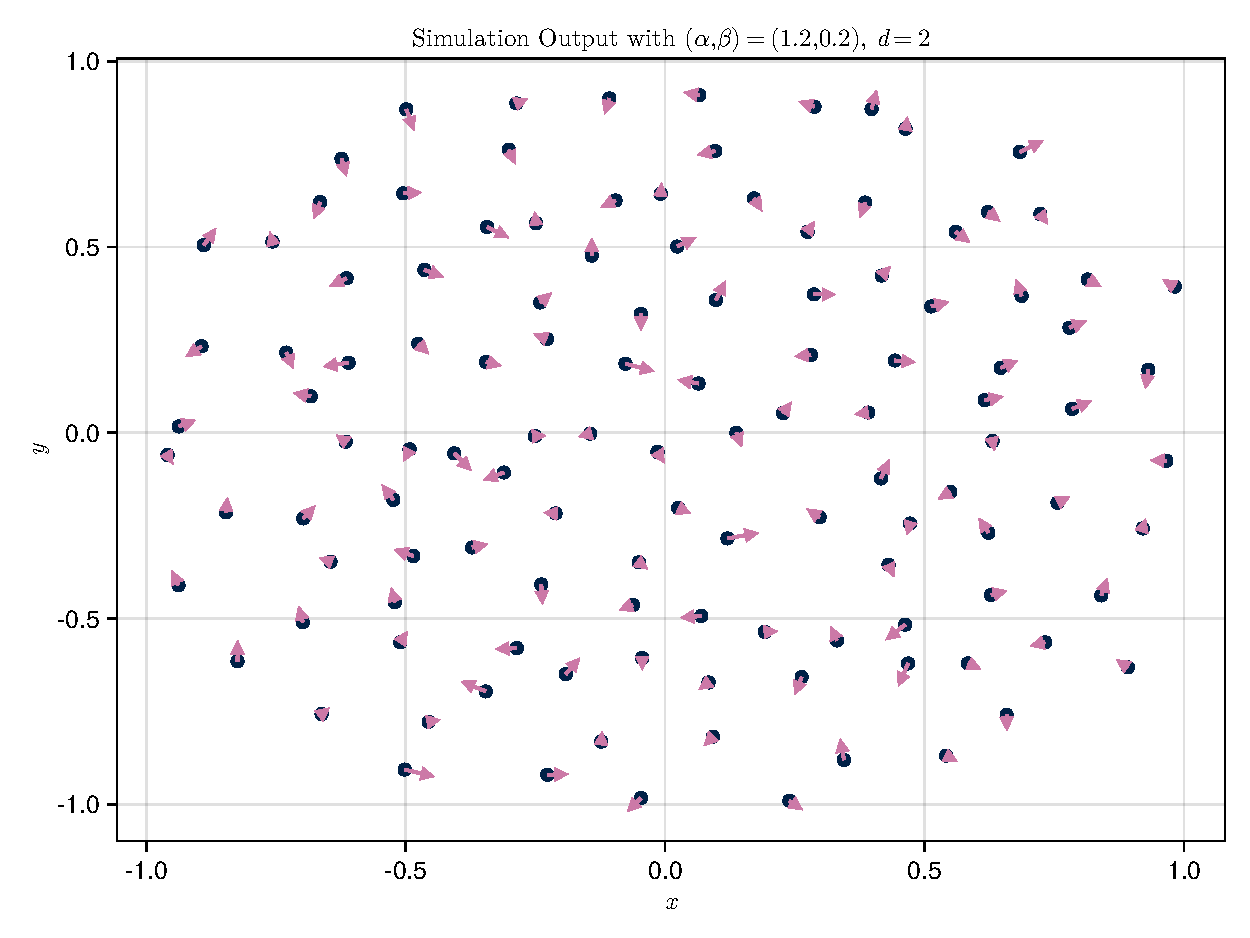
\includegraphics[width=0.8\linewidth]{results/simulation-quiver.pdf}
  \caption{Position and velocity of particles in the simulation at a point in time. Every particle, each of equal mass $m$, interacts with every other particle through the interaction potential $U_{ij} = K\left(\norm{\vec{x_i} - \vec{x_j}}\right)$ leading to $\mathcal{O}(N_p^2)$ interactions.}
\end{figure}

Because each particle interacts with every other particle, the number of interactions scales with $\mathcal{O}(N_p^2)$,
which can play a prohibitive role in terms of the computation time when increasing the number of particles $N_p \gg 1$.

Within the scope of this thesis, in order to understand the elaborate behaviour of such particle systems and also to verify results from theory and the spectral method, we provide an implementation of a simulator starting from a numerical time integrator in $\R^d$.
In addition to the \textit{headless} simulation software, exporting state and results for treatment by the analysis component, a \gls{gui} is provided to enable live insight into and interaction with the model.

\begin{figure}[H]
  \centering
  \label{fig:gui-screenshot}
  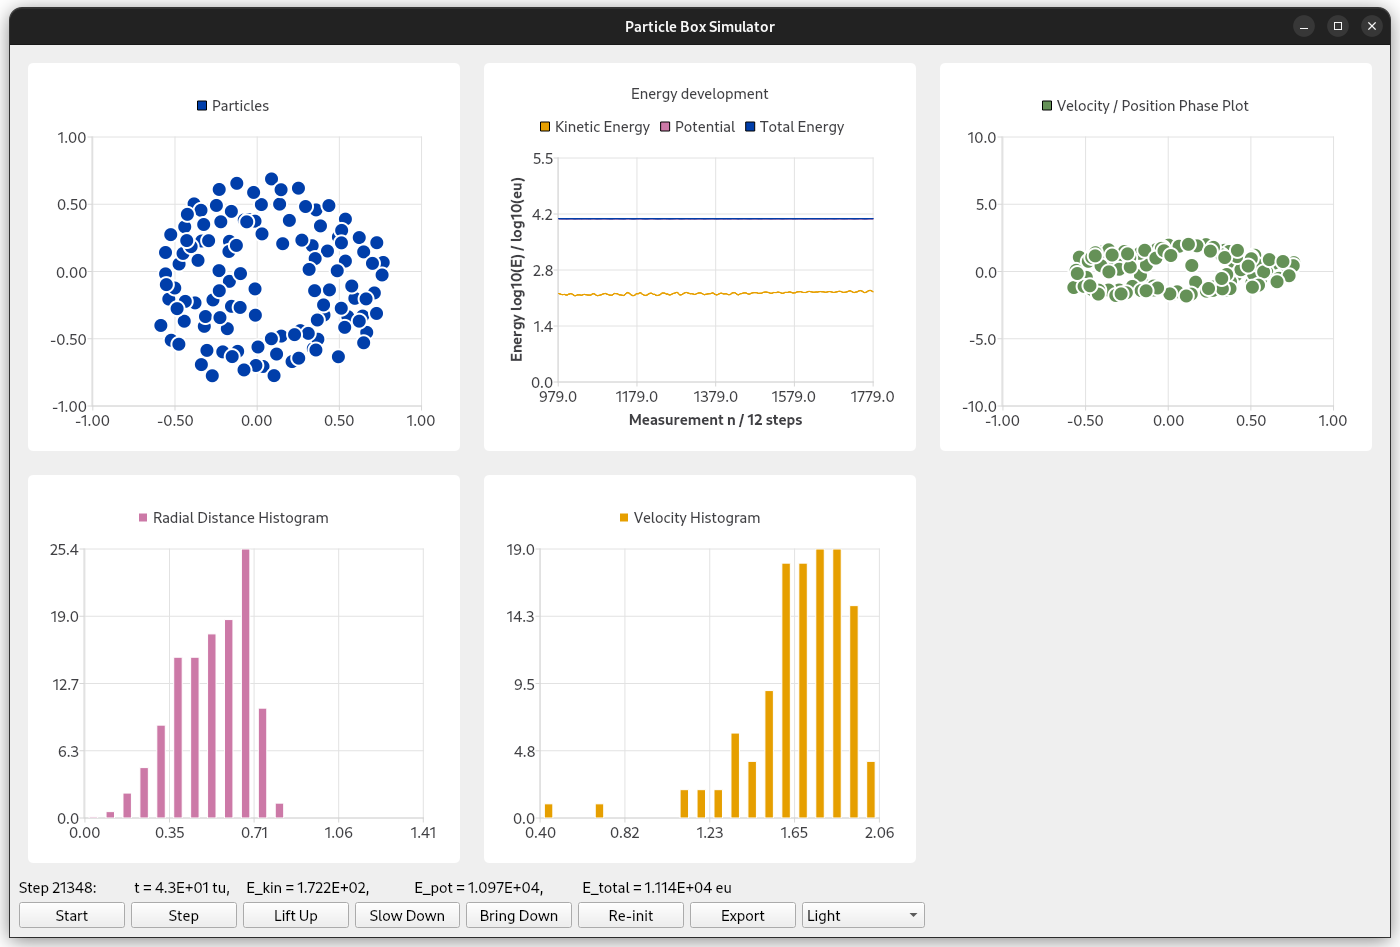
\includegraphics[width=\linewidth]{gui-screenshot.png}
  \caption{Screenshot of the \gls{gui} provided for the particle simulator. The top row shows the position of particles in their $[-1, 1]^d$ domain at a point $t$ in time, the energy development over time and the current position/velocity phase space plot. Below, there are position and velocity histogram updated live along with the simulation.}
\end{figure}

\section{Available Methods}
\begin{itemize}
  \item Simple Forward Integration
  \item Multistep Methods, which is an extension to the simple integration above.
  \item Fast Multipole Method
  \item Multigrid Methods
\end{itemize}

\subsection{Leapfrog Integration}
\input{chapters/out/Leapfrog Integration.md.tex}
\hierKoennteIhreWerbungStehen
% TODO: vielleicht eine kleine Figure zur Visualisierung des Leap-Frogs

\section{Phase Space}
Each particle, at every point in time $t$, has a position and velocity value.
In $d=1$ dimension, one can visualise both of these quantities simultaneously in a phase space plot (cf. \Cref{fig:phase-space-plot}).
For $d > 1$ dimension, it is possible to either only visualise the first components $\{\vec{x_i}\}_1$ and $\{\vec{v_i}\}_1$ or to visualise the norm of the position (distance from the center of mass) $\norm{\vec{x_i} - \vec{x}_{\text{center}}}$ and velocity $\norm{\vec{v_i}}$, where $$\vec{x}_{\text{center}} := \frac{1}{N_p} \sum_{i=1}^{N_p} \vec{x_i}\,.$$

\begin{figure}[H]
  \centering
  \label{fig:phase-space-plot}
  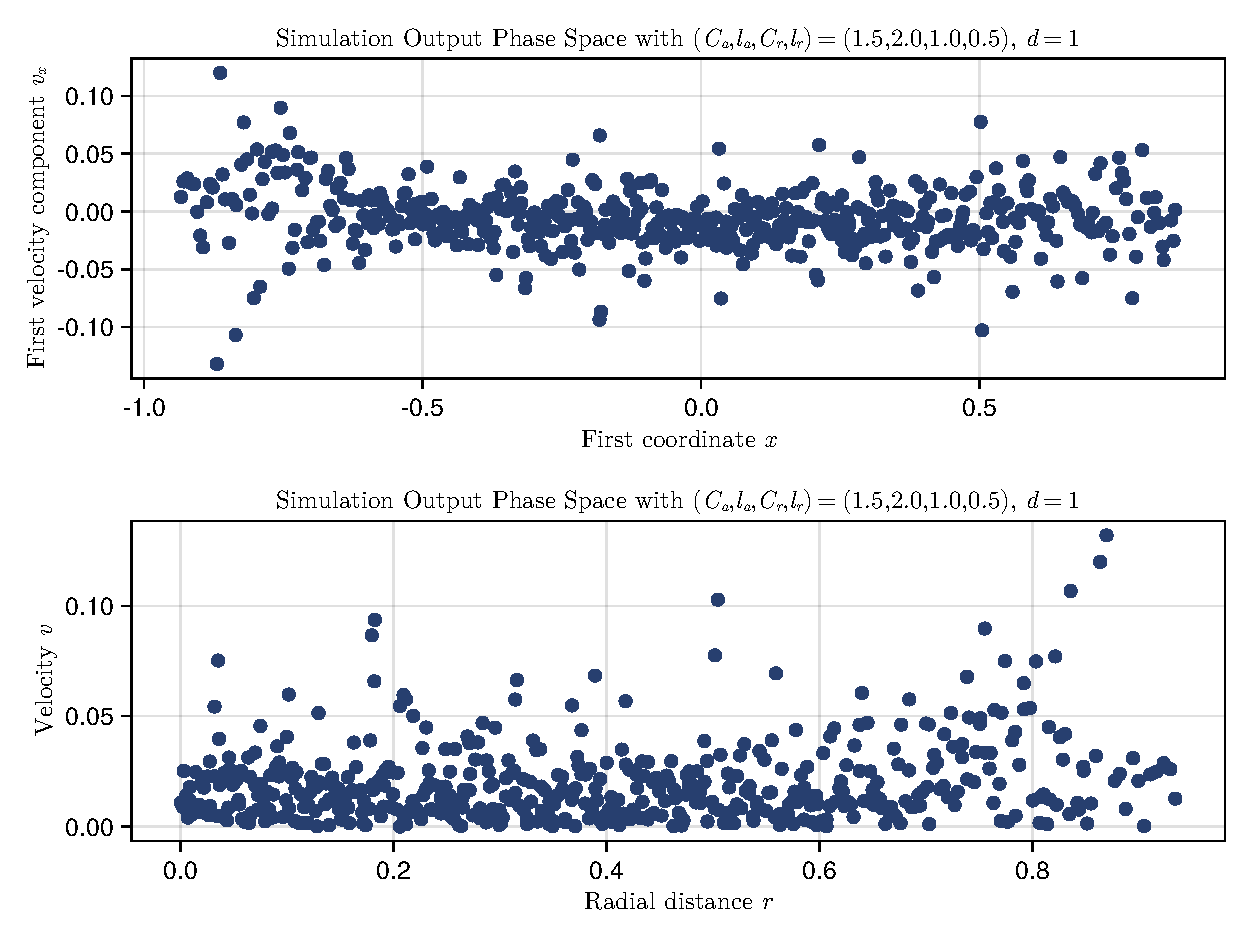
\includegraphics[width=0.8\linewidth]{results/phase-space-plot.pdf}
  \caption{Position and velocity of particles in the simulation visualised as a phase space plot.}
\end{figure}

\begin{figure}[H]
  \centering
  \label{fig:simulation-histogram}
  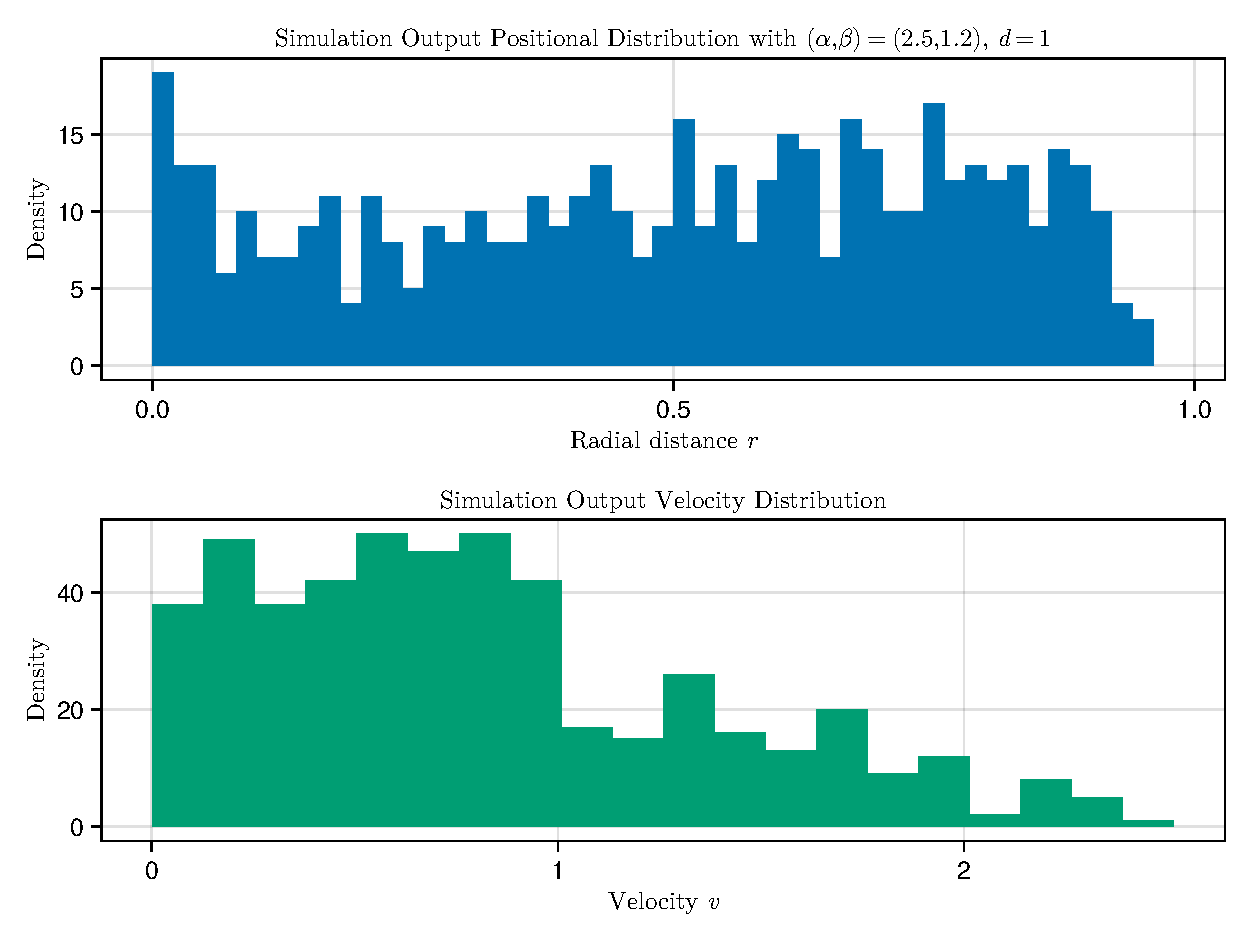
\includegraphics[width=0.8\linewidth]{results/simulation-histogram.pdf}
  \caption{Position Histogram}
\end{figure}
